% #############################################################################    % This is the MAIN DOCUMENT of the IST-UL-Project-Report TEMPLATE. 
% !TEX root = ./main.tex
% #############################################################################
% The document is automatically set for english or portuguese by just selecting
% the MAIN LANGUAGE in file 'IST-UL-Project-Report-Preamble.tex' 
% #############################################################################
% Version 1.0, October 2018
% BY: Prof. Rui Santos Cruz, rui.s.cruz@tecnico.ulisboa.pt
% #############################################################################
% Set the document class
% ----------------------------------------------------------------------
\documentclass[12pt,a4paper]{report}
\usepackage{latexsym}

% -----------------------------------------------------------------------------
% The Preamble document contains all the necessary Packages for typesetting
% Modify it to suit your needs
% -----------------------------------------------------------------------------
% #############################################################################
% Preamble for IST-UL-Project-Report in English or Portuguese
% Required Packages and commands
% --> Please Choose the MAIN LANGUAGE for the Thesis in package BABEL (below)
% !TEX root = ./main.tex
% #############################################################################
% Version 1.0, October 2018
% BY: Prof. Rui Santos Cruz, rui.s.cruz@tecnico.ulisboa.pt
% ######################+OPTIONS: tex:t########################################################
% -----------------------------------------------------------------------------
% PACKAGE ucs:
% -----------------------------------------------------------------------------
% The 'ucs' package provides support for using UTF-8 in LaTeX documents. 
% However in most situations it is not required.
\usepackage{ucs}
% -----------------------------------------------------------------------------
% PACKAGE utf8x:
% -----------------------------------------------------------------------------
% The 'utf8x' package contains support for using UTF-8 as input encoding. 
\usepackage[utf8x]{inputenc}
% -----------------------------------------------------------------------------
% PACKAGE babel:
% -----------------------------------------------------------------------------
% The 'babel' package may correct some hyphenation issues of LaTeX. 
% Select your MAIN LANGUAGE for the Thesis with the 'main=' option.
% 
\usepackage[main=english]{babel}
% -----------------------------------------------------------------------------
% PACKAGE iflang:
% -----------------------------------------------------------------------------
% The 'iflang' package is used to help determine the language being used. 
\usepackage{iflang}
% -----------------------------------------------------------------------------
% PACKAGE graphicx:
% -----------------------------------------------------------------------------
% The 'graphicx' package allows that pdf files can be inserted. 
\usepackage{graphicx}

\usepackage{glossaries}
% ----------------------#+OPTIONS: tex:t------------------------------------------------
% Define default and cover page fonts.
% ----------------------------------------------------------------------
% Use Arial font as default
%
\usepackage{mathptmx}

\renewcommand{\rmdefault}{ptm}
\renewcommand{\sfdefault}{ptm}
\def\FontLn{% 16 pt normal
  \usefont{T1}{ptm}{m}{n}\fontsize{16pt}{16pt}\selectfont}
\def\FontLb{% 16 pt bold
  \usefont{T1}{ptm}{b}{n}\fontsize{16pt}{16pt}\selectfont}
\def\FontMn{% 14 pt normal
  \usefont{T1}{ptm}{m}{n}\fontsize{14pt}{14pt}\selectfont}
\def\FontMb{% 14 pt bold
  \usefont{T1}{ptm}{b}{n}\fontsize{14pt}{14pt}\selectfont}
\def\FontSn{% 12 pt normal
  \usefont{T1}{ptm}{m}{n}\fontsize{12pt}{12pt}\selectfont}
% ----------------------------------------------------------------------
% Define page margins and line spacing.
% ----------------------------------------------------------------------
% > set the page margins (2.5cm minimum in every side, as per IST rules)
%
\usepackage{geometry}	
\geometry{verbose,tmargin=2.5cm,bmargin=2.5cm,lmargin=2.5cm,rmargin=2.5cm}
%
% > allow setting line spacing (line spacing of 1.5, as per IST rules)
%
\usepackage{setspace}
\renewcommand{\baselinestretch}{1.5}
% ----------------------------------------------------------------------
% Include external packages.
\usepackage{graphicx}
\usepackage{amsmath}  % AMS mathematical facilities for LaTeX.
\usepackage{amsthm}   % Typesetting theorems (AMS style).
\usepackage{amsfonts} % 
\usepackage{subfigure}
\usepackage{subfigmat}
\usepackage{dcolumn}
\newcolumntype{d}{D{.}{.}{-1}} % column aligned by the point separator '.'
\newcolumntype{e}{D{E}{E}{-1}} % column aligned by the exponent 'E'
\usepackage[pdftex]{hyperref} % enhance documents that are to be
                              % output as HTML and PDF
\hypersetup{colorlinks,       % color text of links and anchors,
                              % eliminates borders around links
            linkcolor=blue,  % color for normal internal links
            anchorcolor=black,% color for anchor text
            citecolor=cyan,  % color for bibliographical citations
            filecolor=black,  % color for URLs which open local files
            menucolor=black,  % color for Acrobat menu items
            urlcolor=teal,   % color for linked URLs
	        bookmarksopen=true,    % don't expand bookmarks
	        bookmarksnumbered=true, % number bookmarks
            }
\usepackage[figure,table]{hypcap}
\usepackage[format=hang,labelfont=bf,font=small]{caption} 
\usepackage{cite}
\usepackage[printonlyused]{acronym}
\usepackage{lipsum}

% -----------------------------------------------------------------------------
% PACKAGE Cleveref:
% -----------------------------------------------------------------------------
% Clever Referencing of document parts
% Note: portuguese is supported through "brazilian" option
\usepackage[\IfLanguageName{english}{english}{brazilian}]{cleveref}
% -----------------------------------------------------------------------------
% PACKAGES xcolor, color
% -----------------------------------------------------------------------------
% These packages are required for list code snippets.
\usepackage{xcolor}
\usepackage{color}
% The following special color definitions are used in the IST Thesis
\definecolor{forestgreen}{RGB}{34,139,34}
\definecolor{orangered}{RGB}{239,134,64}
\definecolor{lightred}{rgb}{1,0.4,0.5}
\definecolor{orange}{rgb}{1,0.45,0.13}	
\definecolor{darkblue}{rgb}{0.0,0.0,0.6}
\definecolor{lightblue}{rgb}{0.1,0.57,0.7}
\definecolor{gray}{rgb}{0.4,0.4,0.4}
\definecolor{lightgray}{rgb}{0.95, 0.95, 0.95}
\definecolor{darkgray}{rgb}{0.4, 0.4, 0.4}
\definecolor{editorGray}{rgb}{0.95, 0.95, 0.95}
\definecolor{editorOcher}{rgb}{1, 0.5, 0} % #FF7F00 -> rgb(239, 169, 0)
\definecolor{chaptergrey}{rgb}{0.6,0.6,0.6}
\definecolor{editorGreen}{rgb}{0, 0.5, 0} % #007C00 -> rgb(0, 124, 0)
\definecolor{olive}{rgb}{0.17,0.59,0.20}
\definecolor{brown}{rgb}{0.69,0.31,0.31}
\definecolor{purple}{rgb}{0.38,0.18,0.81}




\usepackage{listings}
\lstset{escapeinside={<@}{@>}}
\usepackage{minted}

\lstdefinestyle{commandline} {%
language={[WinXP]command.com},
breaklines=true,
%aboveskip=\baselineskip,
belowskip=\baselineskip,
showstringspaces=false,
backgroundcolor=\color{black},
basicstyle=\small\color{white}\ttfamily
showstringspaces=false,
keywordstyle=\color{cyan}\bfseries,
stringstyle=\color{gray}\ttfamily,
commentstyle=\color{green}\itshape,
moredelim=[s][\color{yellow}\bfseries]{C:}{\>}
}

\lstdefinestyle{Bash} {%
language=bash,
breaklines=true,
belowskip=\baselineskip,
backgroundcolor=\color{lightgray},
showstringspaces=false,
keywordstyle=\color{black}\bfseries,
basicstyle=\small\color{black}\ttfamily,
stringstyle=\color{editorOcher}\ttfamily,
commentstyle=\color{brown}\itshape,
otherkeywords={xcode-select, mkdir,rm},
moredelim=[s][\color{darkblue}]{~$},
literate={~} {$\sim$}{1}
}

\lstdefinestyle{Rubytext} {%
language=Ruby,
breaklines=true,
belowskip=\baselineskip,
basicstyle=\small\ttfamily\color{black},
backgroundcolor=\color{lightgray},
showstringspaces=false,
commentstyle = \ttfamily\color{red},
keywordstyle=\ttfamily\color{blue},
stringstyle=\color{orange}
}
\lstset{escapeinside={<@}{@>}}

\lstdefinestyle{py} {%
	language=python,
	literate=%
	*{0}{{{\color{red}0}}}1
	{1}{{{\color{red}1}}}1
	{2}{{{\color{red}2}}}1
	{3}{{{\color{red}3}}}1
	{4}{{{\color{red}4}}}1
	{5}{{{\color{red}5}}}1
	{6}{{{\color{red}6}}}1
	{7}{{{\color{red}7}}}1
	{8}{{{\color{red}8}}}1
	{9}{{{\color{red}9}}}1,
	basicstyle=\small\ttfamily,
	numbers=left,
	% numberstyle=\tiny,
	% stepnumber=2,
	numbersep=5pt,
	tabsize=4,
	extendedchars=true,
	breaklines=true,
	keywordstyle=\color{blue}\bfseries,
	frame=b,
	commentstyle=\color{brown}\itshape,
	stringstyle=\color{editorOcher}\ttfamily,
	showspaces=false,
	showtabs=false,
	xleftmargin=17pt,
	framexleftmargin=17pt,
	framexrightmargin=5pt,
	framexbottommargin=4pt,
	backgroundcolor=\color{lightgray},
	showstringspaces=false,
}










% DEFINE COMMAND FOR: Degree Title depending on language
\newcommand{\tlangDegree}{\IfLanguageName{english}{Computer Science and Engineering}{Engenharia Informática e de Computadores}}
% DEFINE COMMAND FOR: Course Title depending on language
\newcommand{\tlangCourse}{\IfLanguageName{english}{Databases}{Bases de Dados}}
%%%%%%%%%%%%%%%%%%%%%%%%%%%%%%%%%%%%%%%%%%%%%%%%%%%%%%%%%%%%%%%%%%%%%%%%



% \newglossaryentry{ic1}{name=IC-1, description={oordinated Uiersal Time}}

% \newglossaryentry{ic2}{name=IC-2, description={ordinatedUniversal Time}}

% \newglossaryentry{ic3}{name=IC-3, description={oordinatedUnivrsal Time}}

% \newglossaryentry{ic4}{name=IC-4, description={oordinatd Uiversal Time}}

% \newglossaryentry{ic5}{name=IC-5, description={oordinaed Universal Time}}

% \newglossaryentry{ic6}{name=IC-6, description={oordinated Universal Time}}

% \newglossaryentry{ic7}{name=IC-7, description={oordinted Univeral Time}}

% \newglossaryentry{ic8}{name=IC-8, description={oordinated Univeral Time}}

% \newglossaryentry{ic9}{name=IC-9, description={oordinated Universal Time}}

% \makenoidxglossaries



% \newglossaryentry{maths}
% {
% name=mathematics,
% description={Mathematics is what mathematicians do}
% }

%   \newglossaryentry{latex}
%   {
%   name=latex,
%   description={Is a markup language specially suited for 
%   scientific documents}
% }


%   \newglossaryentry{formula}
%   {
%   name=formula,
%   description={A mathematical expression}
% }
%   #############################################################################
\begin{document}



% Set plain page style (no headers, footer with centered page number)
\pagestyle{plain}
% Set roman numbering (i,ii,...) before the start of chapters
\pagenumbering{roman}
% ----------------------------------------------------------------------------
% Cover page
% #############################################################################     % This is the FRONT COVER of the IST-UL-Project-Report TEMPLATE. 
% !TEX root = ./main.tex
% #############################################################################
% Version 1.0, October 2018
% BY: Prof. Rui Santos Cruz, rui.s.cruz@tecnico.ulisboa.pt
% #############################################################################
% #############################################################################
% DO NOT CHANGE THE FOLLOWING 4 LINES
\thispagestyle {empty}

\includegraphics[width=5cm]{./pictures/IST_A_RGB_POS.png}
\begin{center}
\vspace{5.0cm}
% #############################################################################
% #############################################################################
%
% INSERT THE TITLE OF THE PROJECT HERE
{\FontLb DB Project} \\
\vspace{0.2cm}
%
% INSERT THE SUBTITLE OF THE REPORT HERE
{\FontMn Part 2} \\
\vspace{1.0cm}
{\FontLn \tlangCourse} \\
\vspace{0.3cm}
{\FontMn Prof. Ana Cláudia Madeira David} \\
\vspace{0.5cm}
\textbf{Group nr.:}: 177 \\
\begin{center}
\begin{table}[h!]
\centering
\textbf{Total Effort}: 21 hours \\
\vspace{0.6cm}
\begin{tabular}{||c c c||} 
 \hline
 Student's Number & Full Name & Relative effort  \\ [0.5ex] 
 \hline\hline
       96098: & Tomás Gonçalves Lopes Costa Carvalho & 33\% \\
       99078: & Guilherme Henrique Corrêa Carabalone & 33\% \\
       99095: & João Paulo Melo Furtado & 33\% \\

 \hline
\end{tabular}
\caption{Students from the 'BDL05' shift.}
\end{table}
\end{center}
% \begin{center}
% \begin{tabular}{r@{~}l l}
%     \multicolumn{3}{c}{\bfseries\textbf{ }} \\
%     % INSERT YOUR TEAM NUMBER HERE
%     & \textbf{Grupo nr.}: & 177 \\
%     & \textbf{Turno nr.}: & 5 \\
%     % INSERT IDs and NAMES of STUDENTS
    
%     & Número de Aluno & Nome & Esforço Relativo \\
%     & 96098: & Tomás Gonçalves Lopes Costa Carvalho \\
%     & 99078: & Guilherme Henrique Corrêa Carabalone \\
%     & 99095: & João Paulo Melo Furtado \\
% \end{tabular}
% \end{center}
\vspace{2.0cm}
{\FontMb \tlangDegree} \\
{\FontMb IST-TAGUSPARK} \\
\vspace{1.5cm}
{\FontMb 2021/2022} \\
\end{center}
\cleardoublepage
% ----------------------------------------------------------------------------
% Table of contents, list of tables, list of figures and nomenclature
% ----------------------------------------------------------------------------
% Set arabic numbering (1,2,...) after preface
\setcounter{page}{1}
\pagenumbering{arabic}
% #############################################################################
% 
% BEGIN MAIN DOCUMENT BODY
% 
% #############################################################################

% \section*{Entity-Association Modelation}

% \begin{figure}[htpb]
%   \centering
%   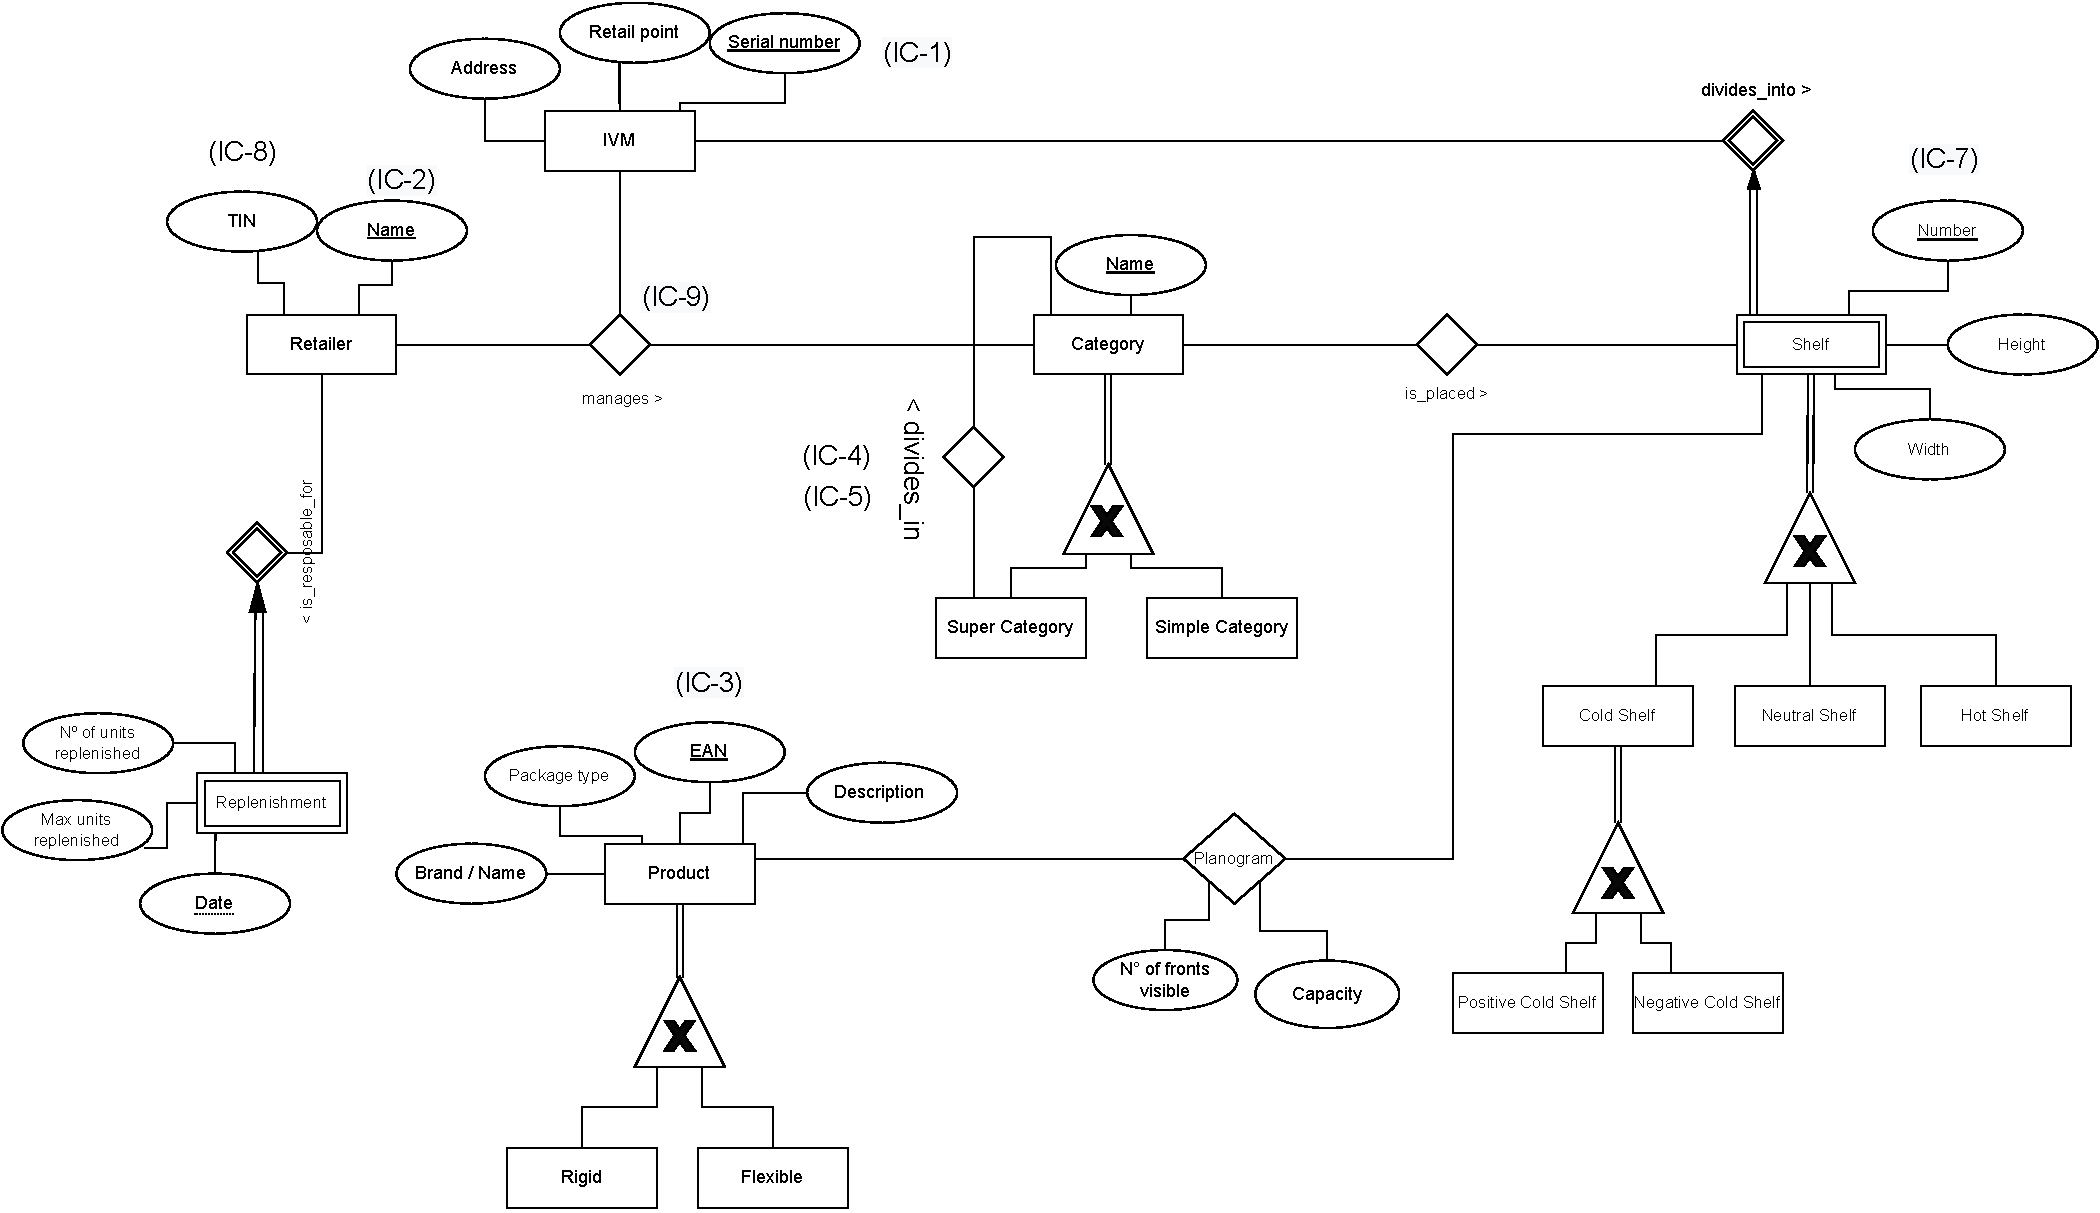
\includegraphics[width=1.0\textwidth]{./pictures/cona.pdf} 
%   \caption{The modelation of the problem, regarding the Entity-Association modelation's theory.}.
% \end{figure}

% % \gls

% % \printnoidxglossaries
% \subsection*{Integrity Constraints}

% \begin{itemize}
% \item (IC-1) A Category cannot be contained in itself.

% \item (IC-2) Cannot exist cycles on the hierarchy of Categories.

% \item (IC-3) The name of the Retailer is unique.

% \item (IC-4) The number of units replenished in a singular event of Replenishement cannot exceed the number of units specified on the Planogram.

% \item (IC-5) A Product can only be replenished in a Shelf where its category is noted.

% \item (IC-6) A Product can only be replenished by the Retailer responsible by Products's category.

% \end{itemize}

\section*{Relational Model}

\begin{itemize}
  
\item point\_of\_retail(\underline{address}, name).

\item IVM(\underline{serial\_number}, \underline{manuf})
  
\item product(\underline{EAN}, descr)
  \begin{itemize}
  \item shelf(\underline{serial\_number}, \underline{manuf}, \underline{nr}, height)
  \item serial\_number: FK(IVM)
  \item manuf: FK(IVM)
  \end{itemize}

\item ambient\_temp\_shelf(\underline{nr})
  \begin{itemize}
  \item nr: FK(shelf)
  \end{itemize}

\item warm\_shelf(\underline{nr})
  \begin{itemize}
  \item nr: FK(shelf)
  \end{itemize}
  
\item cold\_shelf(\underline{nr})
  \begin{itemize}
  \item nr: FK(shelf)
  \end{itemize}

\item category(\underline{name})
  
\item simple\_category(\underline{name})
  \begin{itemize}
  \item name: FK(shelf)
  \end{itemize}

\item super\_category(\underline{name})
  \begin{itemize}
  \item name: FK(shelf)
  \end{itemize}

\item retailer(\underline{TIN}, name)
  \begin{itemize}
  \item UNIQUE(name)
  \end{itemize}
  
\item replenishment\_event(\underline{instant}, units)
  
\item installed-at(address, \underline{serial\_number}, \underline{manuf}, nr)
  \begin{itemize}
  \item address: FK(point\_of\_retail)
  \item serial\_number: FK(IVM)
  \item manuf: FK(IVM)
    \end{itemize}

\item replenisher\_of(\underline{TIN}, \underline{instant})
  \begin{itemize}
  \item TIN: FK(retailer)
  \item instant: FK(replenishment\_event)
  \end{itemize}
  
\item replenishment(\underline{instant}, \underline{EAN}, \underline{nr})
  \begin{itemize}
  \item instant: FK(replenishment\_event)
  \item EAN: FK(planogram.EAN, planogram.nr)
  \item nr: FK(planogram.EAN, planogram.nr)
  \end{itemize}
  
\item has(\underline{EAN}, \underline{name})
  \begin{itemize}
  \item EAN: FK(product)
  \item name: FK(category)
    \end{itemize}


\item planogram(\underline{EAN}, \underline{nr}, faces, units, loc)

\item responsable\_for(\underline{name}, \underline{TIN}, \underline{serial\_number}, \underline{manuf})
  \begin{itemize}
  \item name: FK(category)
  \item TIN: FK(retailer)
  \item serial\_number: FK(IVM)
  \item manuf: FK(IVM)
  \end{itemize}
  
\item displayed(\underline{name}, \underline{nr})
  \begin{itemize}
  \item name: FK(category)
  \item nr: FK(category)
  \end{itemize}

\item of(\underline{nr}, \underline{serial\_number}, \underline{manuf})
  \begin{itemize}
  \item nr: FK(shelf)
  \item serial\_number: FK(IVM)
  \item manuf: FK(IVM)
  \end{itemize}

\item has-other(\underline{category\_name}, \underline{super\_category\_name})
  \begin{itemize}
  \item category\_name: FK(category.name)
  \item super\_category\_name: FK(category.name)
  \end{itemize}

\end{itemize}
% \item (IC-1) A Category cannot be contained in itself.

% \item (IC-2) Cannot exist cycles in the hierarchy of Categories.

% \item (IC-3) The name of the Retailer is unique.

% \item (IC-4) The number of units replenished in a singular event of Replenishement cannot exceed the number of units specified on the Planogram. The number of units from Replenishment event is always less or equal than the number of units in the Planogram.

% \item (IC-5) A Product can only be replenished in a Shelf where its category is noted.

% \item (IC-6) A Product can only be replenished by the Retailer responsible by Products's category.

\section*{Integrity Constraints}
\subsection*{Relational Model}
\begin{itemize}
\item (IC-1): category\_name is always different from super\_category\_name.
\item (IC-2): Cannot exist cycles in the hierarchy of Categories.
\item (IC-3): The number of units replenished in a singular event of Replenishement cannot exceed the number of units specified on the Planogram.
\item (IC-4): A Product can only be replenished in a Shelf where its category is noted.
\item (IC-5): A Product can only be replenished by the Retailer responsible by Products's category.
\item (IC-6): A name can only exist in simple\_category or super\_category.
\item (IC-7): Every product (EAN) must participate in the has associaton.
\item (IC-8): EAN can only exist in ambient\_temp\_shelf, warm\_shelf or cold\_shelf.
\end{itemize}



\section*{Relational Algebra}
\begin{enumerate}
\item[1.] $\pi_{EAN, designacao}(\sigma_{name = "Barras\ de\ Energetico" \land  instant > "2021/12/31" \land units > 10 }(Product \Join Replenishment Event))$
\item[2.] $\pi_{serial\_number}(\sigma_{EAN = 9002490100070})((Products \Join Planogram)\Join of)$
\item[3.] $G_{count}() \rightarrow_{c(has-other)}(\sigma_{name = "SopasTake-Away"}(category))$
\item[4.] $prods \leftarrow _{EAN, Designacao}G_{count() \rightarrow c(replenishment)}$ \\
  $result \leftarrow G_{max(c)}(prods) \Join prods$
\end{enumerate}

\section*{SQL}
\begin{enumerate}
\item[1.]
\begin{verbatim}
SELECT ean, descr
    FROM product NATURAL JOIN Replenishment_Event
    WHERE name = "Barras de Energético"
        AND instant > "2021/12/31"
        AND units > 10;
\end{verbatim}
\item[2.]
\begin{verbatim}
SELECT serial_number
    FROM Products NATURAL JOIN Planogram NATURAL JOIN of
    WHERE ean = 9002490100070; 
\end{verbatim}

\item[3.]
\begin{verbatim}
SELECT COUNT(category_name)
    FROM has-other
    WHERE super_category_name = "SopasTake-Away";
\end{verbatim}

\item[4.]
  \begin{verbatim}
SELECT ean, descr
FROM (
    SELECT ean, descr, COUNT(instant)
    FROM product NATURAL JOIN replenishment
    GROUP BY ean, descr
) AS table
WHERE count >= ALL (
    SELECT count
    FROM table
);
    

\end{verbatim}
\end{enumerate}
\end{document}